\documentclass[../main.tex]{subfiles}
\begin{document}
\section{对抗搜索与多智能体博弈}\label{sec:adversarial-search}
\subsection{博弈的理论框架：对抗搜索}\label{sec:game-framework}
\begin{enumerate}
    \item \textbf{博弈的基本概念与博弈类型}
    \begin{itemize}
        \item \textbf{非合作博弈：}竞争环境中多个agent之间的目标是有冲突的，称为对抗搜索问题，也称为博弈(Games)，或者非合作博弈
        \item \textbf{合作博弈：}智能体相互合作以获得最大回报也是博弈的一种，称为合作博弈
    \end{itemize}
    \item \textbf{均衡理论}
    \begin{itemize}
        \item \textbf{均衡：}博弈中所有参与者都不想改变自己的策略的这样一种相对静止的状态\footnote{对抗搜索的目标是寻找最优策略，而均衡理论证明该策略的稳定性}
        \item \textbf{均衡理论分类}
        \begin{itemize}
            \item 
        \end{itemize}
        \item \textbf{纳什均衡：}又称非合作博弈均衡，每个博弈者的平衡策略都是为了达到自己期望收益的最大值，与此同时，其他所有博弈者干遵循这样的策略。
        \begin{itemize}
            \item \textbf{支配性策略：}在一个博弈过程中，无论对方的策略选择如何，当事人一方都会选择某个确定的策略，则该策略被称作支配性策略。
            \item \textbf{纳什均衡：}如果任意一位参与者在其他所有参与者的策略确定的情况下，其选择的策略是最优的，那么这个组合就被定义为纳什平衡
            \item \textbf{性质：}纳什均衡是完全理性、非合作、静态、完全信息博弈的基准解
            \item \textbf{举例：}囚徒困境
        \end{itemize}

        
    \end{itemize}
\end{enumerate}
\subsection{极大极小与剪枝算法}\label{sec:minimax-alpha-beta}
\begin{enumerate}
    \item \textbf{极大极小算法(minimax)原理与递归求值}
    \begin{itemize}
        \item \textbf{应用场景：}两人零和博弈（e.g. 井字棋、象棋）
        \item \textbf{核心思想：}
        \begin{itemize}
            \item \textbf{两个角色：}MAX（我方，让自己最终得分最大化）和MIN（对手，让我方最终得分最小化）
            \item \textbf{核心假设：}假设对手和我们一样聪明，他每一步都会选择对自己最有利（对我们最不利）的走法
            \item \textbf{我们的策略：}在所有可能的走法中，选择一条路，即使在这条路上被对手“围追堵截”(让他选了最小值)，我们最终能拿到的保底收益依然是所有路线里最大的
        \end{itemize}
        \item \textbf{原理：} MAX将优先选择移动到一个具有极大值的状态，MIN则选择移动到极小值的状态，使用简单递归算法，计算每个后继的极小极大值
        \begin{figure}[H]
            \centering
            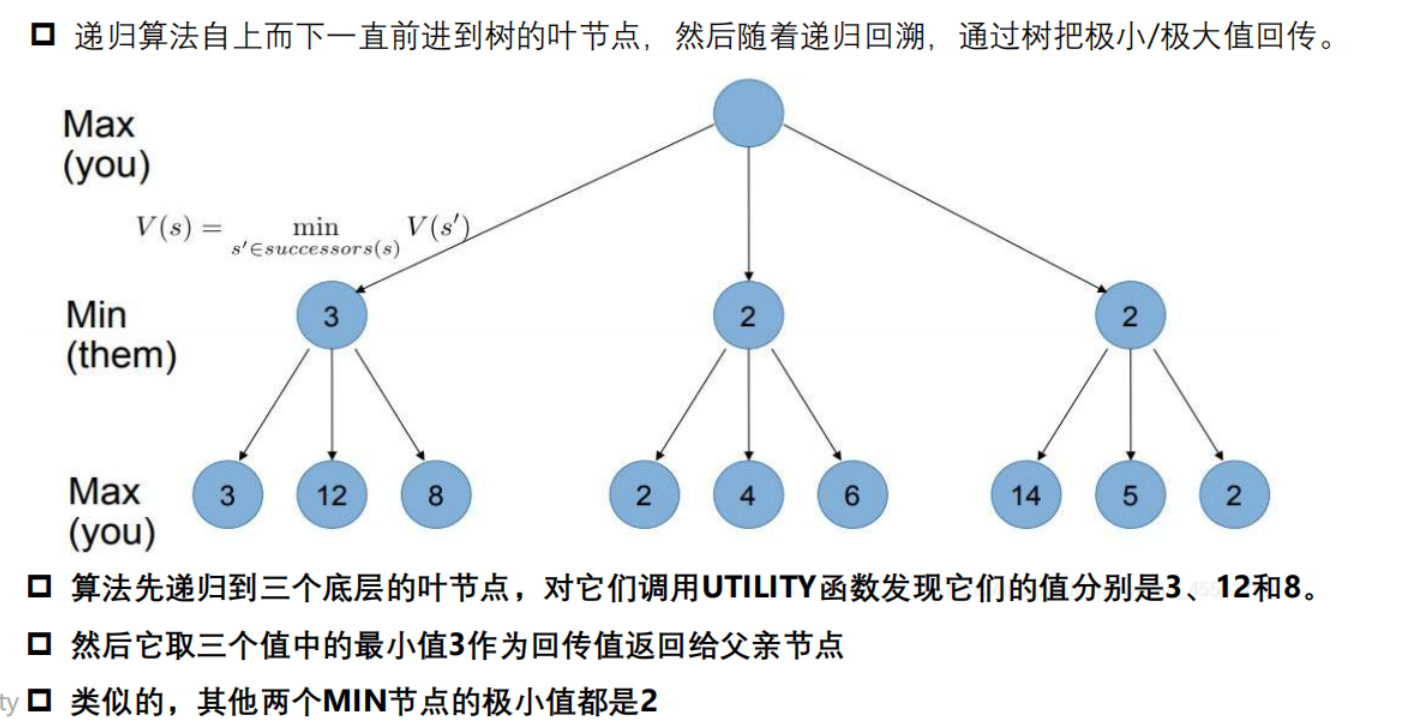
\includegraphics[width=0.75\linewidth]{images/maxmin.png}
            \caption{极大极小算法原理实例}
            \label{fig:placeholder}
        \end{figure}
    \end{itemize}
      \item \textbf{$\alpha-\beta$剪枝}
    \begin{itemize}
        \item \textbf{推荐资料：}\href{https://oi-wiki.org/search/alpha-beta/}{OI Wiki：Alpha-Beta 剪枝}；\href{https://www.bilibili.com/video/BV1a7411K7g1/?spm_id_from=333.1007.top_right_bar_window_default_collection.content.click&vd_source=5deca47094767260f853b759a625a68f}{B站视频讲解}\footnote{这两份资料都很不错，所以我就不整理具体算法了，实际上该算法几乎是\textcolor{red}{必考}，所以请务必理解并学会使用}
        \item \textbf{地位：}对minimax方法的优化，结果完全相同，只是运行效率更高
        \item \textbf{基本思想：}根据上一层已经得到的当前最优结果，决定目前的搜索是否要继续下去\footnote{当你知道你有一个选择A时，此时你知道了B选择不如A选择好，那么你就不需要知道B选择有多坏。}。
        \item \textbf{两个假设：}零和博弈、双方聪明
    \end{itemize}
    \item \textbf{改进算法}
   \begin{itemize}
        \item \textbf{动机：}$\alpha-\beta$剪枝虽提高了搜索效率，但完全搜索到终止状态仍不现实，因此需要进一步近似。
        \item \textbf{改进方法：}评估函数与截断搜索。
        \begin{itemize}
            \item \textbf{评估函数：}
            \begin{itemize}
                \item 应与真正的效用函数对终止状态给出相同排序；
                \item 计算应足够快；
                \item 对非终止状态，应尽量与实际胜率相关；
                \item 在计算能力有限时，本质上是对最终结果的近似预测；
                \item 常通过提取状态特征并做加权求和来构造，国际象棋中常用加权线性函数。
            \end{itemize}

            \item \textbf{截断搜索：}
            \begin{itemize}
                \item \textbf{思想：}不再搜索到终局，而是在预设深度的截断点停止，并用评估函数估计当前局面优劣；
                \item \textbf{原因：}复杂博弈存在组合爆炸，完全搜索计算量不可承受，搜索深度直接影响棋力；
                \item \textbf{问题：}可能出现\textbf{水平线效应}，即在截断点看似平静，但截断点之后可能立刻出现关键变化，导致误判；
                \item \textbf{改进：}采用\textbf{静止搜索（Quiescence Search）}，在达到深度限制后不立即停止，而是继续扩展“动荡”局面，直到局面相对稳定后再调用评估函数，从而减弱水平线效应。
            \end{itemize}
        \end{itemize}
    \end{itemize}
        
\end{enumerate}

\subsection{多智能体博弈}
\textcolor{red}{这一章知道概念就行了，不用细看式子}
\begin{enumerate}
    \item \textbf{体系中的博弈：}
    \begin{itemize}
        \item \textbf{概念：}
        \begin{itemize}
            \item \textbf{多智能体系统（Multi-Agent System, MAS）：}由多个自主智能体组成的分布式系统，每个智能体能够自主感知环境、学习并作出决策，以实现各自目标或协同完成整体目标；
            \item \textbf{多智能体博弈：}多个自主智能体在共同环境中进行竞争或合作，并通过交互和策略调整实现各自或共同目标的过程。
        \end{itemize}

        \item \textbf{博弈任务分类：}
        \begin{itemize}
            \item \textbf{完全合作任务：}所有智能体目标一致，典型例子如仓储机器人；
            \item \textbf{完全竞争任务：}智能体目标相互对立，典型例子如围棋游戏；
            \item \textbf{混合任务：}同时包含合作与竞争，典型例子如机器人足球。
        \end{itemize}

        \item \textbf{序贯决策的三种设置：}
        \begin{itemize}
            \item \textbf{马尔可夫决策过程（MDP）：}一个决策者，多个状态；
            \item \textbf{重复博弈（矩阵博弈）：}多个决策者，一个状态；
            \item \textbf{随机博弈（马尔可夫博弈）：}多个决策者，多个状态。
        \end{itemize}

        \item \textbf{随机博弈（Stochastic Game, SG）：}
        \begin{itemize}
            \item 一个随机博弈具有多个状态和多个智能体；
            \item 每个状态对应一个标准形式博弈；
            \item 每一轮之后，游戏会随机转移到另一个状态；
            \item 转移概率取决于当前状态和所有智能体采取的联合动作；
            \item 通常奖励会随时间打折。
        \end{itemize}

        \item \textbf{随机博弈的定义：}
        一个随机博弈可由如下元组表示：
        $$
        (S,A^1,\ldots,A^N,r^1,\ldots,r^N,p,\gamma)
        $$
        其中：
        \begin{itemize}
            \item \textbf{状态空间：} $S$；
            \item \textbf{智能体 $j$ 的动作空间：} $A^j,\ j\in\{1,\ldots,N\}$；
            \item \textbf{智能体 $j$ 的奖赏函数：}
            $$
            r^j:S\times A^1\times \cdots \times A^N \to \mathbb{R}
            $$
            \item \textbf{转移概率：}
            $$
            p:S\times A^1\times \cdots \times A^N \to \Omega(S)
            $$
            其中 $\Omega(S)$ 表示状态空间 $S$ 上的概率分布集合；
            \item \textbf{时间折扣因子：}
            $$
            \gamma\in[0,1)
            $$
        \end{itemize}

        \item \textbf{随机博弈中的策略与价值：}
        \begin{itemize}
            \item 对于智能体 $j$，其策略为
            $$
            \pi^j:S\to \Omega(A^j)
            $$
            即在动作空间 $A^j$ 上的概率分布；
            \item 所有智能体的联合策略为
            $$
            \pi \triangleq [\pi^1,\ldots,\pi^N]
            $$
            \item 智能体 $j$ 的状态价值函数为
            $$
            v_\pi^j(s)=v^j(s;\pi)=\sum_{t=0}^{\infty}\gamma^t\mathbb{E}_{\pi,p}[r_t^j\mid s_0=s,\pi]
            $$
            \item 智能体 $j$ 的动作价值函数为
            $$
            Q_\pi^j:S\times A^1\times \cdots \times A^N \to \mathbb{R}
            $$
            且
            $$
            Q_\pi^j(s,a)=r^j(s,a)+\gamma \mathbb{E}_{s'\sim p}[v_\pi^j(s')]
            $$
            其中 $a=[a^1,\ldots,a^N]$ 表示联合动作。
        \end{itemize}

        \item \textbf{随机博弈中的独立学习：}
        \begin{itemize}
            \item 若对每个智能体 $j$，假设其他智能体的策略固定，则对它而言环境是固定的，因此可以执行 Q-learning；
            \item 但在多智能体强化学习（MARL）中，每个智能体都在学习并更新策略，因此环境对任一智能体而言通常是非平稳的。
        \end{itemize}

        \item \textbf{随机博弈中的纳什均衡：}
        \begin{itemize}
            \item 智能体的优化目标取决于联合策略 $\pi$；
            \item 随机博弈中的纳什均衡由一个特定的联合策略表示：
            $$
            \pi_* \triangleq [\pi_*^1,\ldots,\pi_*^N]
            $$
            \item 其定义为：在给定其他智能体策略的情况下，没有任何一个智能体愿意单独改变自己的策略，即
            $$
            v^j(s;\pi_*)=v^j(s;\pi_*^j,\pi_*^{-j})\geq v^j(s;\pi^j,\pi_*^{-j})
            $$
            其中
            $$
            \pi_*^{-j}\triangleq[\pi_*^1,\ldots,\pi_*^{j-1},\pi_*^{j+1},\ldots,\pi_*^N]
            $$
        \end{itemize}

        \item \textbf{从多智能体到多智能体强化学习：}
        \begin{itemize}
            \item 当智能体数量增加时，奖励函数与状态转移概率都会随智能体数目呈指数级增长；
            \item 因而多智能体强化学习通常面临：
            \begin{itemize}
                \item 更难建模；
                \item 环境更具动态性和敏感性；
                \item 需要更多探索数据；
                \item 需要更多计算资源。
            \end{itemize}
        \end{itemize}
    \end{itemize}

    \item \textbf{纳什Q-Learning：}
    \begin{itemize}
        \item \textbf{核心思想：}将单智能体 Q-learning 推广到随机博弈中，在每一步学习中引入纳什均衡。
        \item \textbf{纳什价值函数：}给定一个纳什策略 $\pi_*$，纳什价值函数为
        $$
        v^{\mathrm{Nash}}(s)\triangleq [v_{\pi_*}^1(s),\ldots,v_{\pi_*}^N(s)]
        $$
        \item \textbf{基本过程：}
        \begin{itemize}
            \item 先求解由当前 $Q_t$ 定义的当前阶段纳什均衡 $\pi_*$；
            \item 再利用新的纳什值 $v^{\mathrm{Nash}}$ 改进 $Q$ 函数的估计。
        \end{itemize}
        \item \textbf{存在问题：}
        \begin{itemize}
            \item 计算复杂度很高；
            \item 当其他智能体的策略不可用时可能无法工作，即对对手建模要求较强。
        \end{itemize}
    \end{itemize}
\end{enumerate}

\end{document}
